\documentclass[12pt]{article}
%Gummi|065|=)
\usepackage{amsmath, amsfonts, amssymb}
\usepackage[margin=0.5in]{geometry}
\usepackage{xcolor}
\usepackage{graphicx}
\newcommand{\off}[1]{}
\DeclareMathSizes{20}{30}{21}{18}

\newcommand{\bsq}[2]{
\fill[black](#1,#2)--(#1+1,#2)--(#1+1,#2+1)--(#1,#2+1)--cycle;
%\draw[](#1,#2)--(#1+1,#2)--(#1+1,#2+1)--(#1,#2+1)--cycle;
 }
 
\newcommand{\gsq}[2]{
\fill[black!60!white](#1,#2)--(#1+1,#2)--(#1+1,#2+1)--(#1,#2+1)--cycle;
%\draw[](#1,#2)--(#1+1,#2)--(#1+1,#2+1)--(#1,#2+1)--cycle;
 }

\newcommand{\wsq}[2]{
\fill[black!10!white](#1,#2)--(#1+1,#2)--(#1+1,#2+1)--(#1,#2+1)--cycle;
%\draw[](#1,#2)--(#1+1,#2)--(#1+1,#2+1)--(#1,#2+1)--cycle; 
}

\newcommand{\sq}[3]{
\fill[#1] (#2,#3)--(#2+1,#3)--(#2+1,#3+1)--(#2,#3+1)--cycle; }

\newcommand{\myhrule}{}

\usepackage{tikz}

\title{\textbf{ Attempt at: the Arctic Circle Theorem }}
\author{John D Mangual}
\date{}
\begin{document}

\fontfamily{qag}\selectfont \fontsize{25}{30}\selectfont

\maketitle


\noindent 
Domino Tilings is notoriously hard to code and to theorize about at the same time.  All my scrawled pages are lost. \\ \\
Exercise 1: Draw an Aztec Diamond
\begin{center}

\begin{tikzpicture}


\bsq{0}{2}
\wsq{-1}{2}

\bsq{ 1}{ 1}
\wsq{ 0}{ 1}
\bsq{-1}{ 1}
\wsq{-2}{ 1}

\bsq{2}{0}
\wsq{1}{0}
\bsq{0}{0}
\wsq{-1}{0}
\bsq{-2}{0}
\wsq{-3}{0}

\wsq{ 2}{-1}
\bsq{ 1}{-1}
\wsq{ 0}{-1}
\bsq{-1}{-1}
\wsq{-2}{-1}
\bsq{-3}{-1}

\wsq{ 1}{-2}
\bsq{ 0}{-2}
\wsq{-1}{-2}
\bsq{-2}{-2}

\wsq{ 0}{-3}
\bsq{-1}{-3}

\end{tikzpicture}
\end{center} \newpage
Exercise 2: Draw some dominoes

\begin{center}
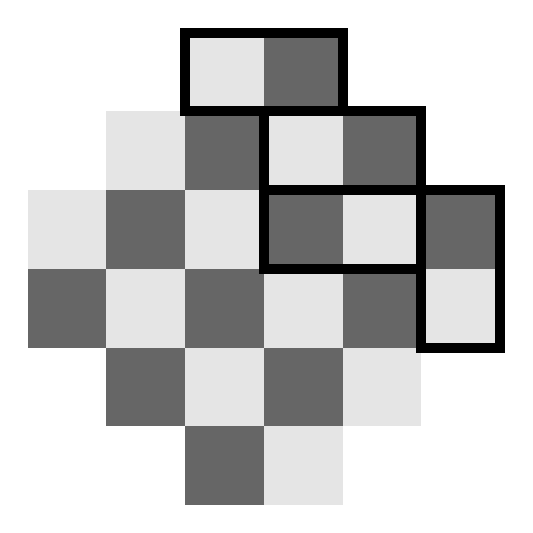
\begin{tikzpicture}


\gsq{0}{2}
\wsq{-1}{2}

\gsq{ 1}{ 1}
\wsq{ 0}{ 1}
\gsq{-1}{ 1}
\wsq{-2}{ 1}

\gsq{2}{0}
\wsq{1}{0}
\gsq{0}{0}
\wsq{-1}{0}
\gsq{-2}{0}
\wsq{-3}{0}

\wsq{ 2}{-1}
\gsq{ 1}{-1}
\wsq{ 0}{-1}
\gsq{-1}{-1}
\wsq{-2}{-1}
\gsq{-3}{-1}

\wsq{ 1}{-2}
\gsq{ 0}{-2}
\wsq{-1}{-2}
\gsq{-2}{-2}

\wsq{ 0}{-3}
\gsq{-1}{-3}

\draw[line width=0.05in] (0,0)--(2,0)--(2,1)--(0,1)--cycle;

\draw[line width=0.05in] (0,1)--(2,1)--(2,2)--(0,2)--cycle;

\draw[line width=0.05in] (-1,2)--(1,2)--(1,3)--(-1,3)--cycle;

\draw[line width=0.05in] (2,1)--(3,1)--(3,-1)--(2,-1)--cycle; 

\end{tikzpicture}
\end{center}
How to encode one domino?  The middle line is at  (1,0) and (1,1) so we will encode it as \texttt{1-0-1}, and we specify that it is horizontal\footnote{We'll always get stuck since there's no language for having one item in \textbf{two} places.  Maybe it's not so bad.  This would be a redundant way to store this information on a computer, but hey we're drawing.  This is a separate problem!}. \\

\noindent Exercise 3: finish the domino tiling

\begin{center}
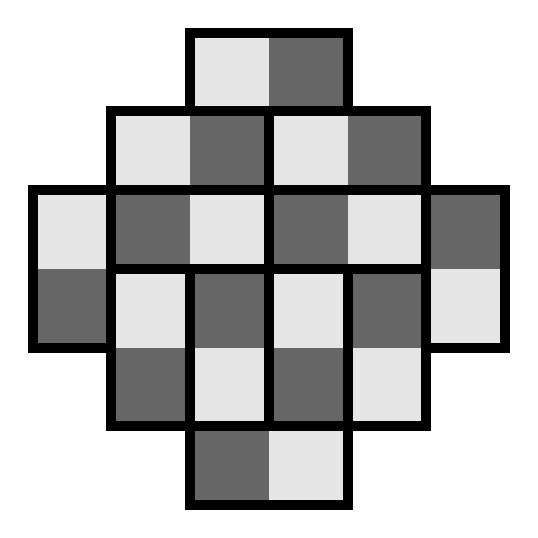
\begin{tikzpicture}


\gsq{0}{2}
\wsq{-1}{2}

\gsq{ 1}{ 1}
\wsq{ 0}{ 1}
\gsq{-1}{ 1}
\wsq{-2}{ 1}

\gsq{2}{0}
\wsq{1}{0}
\gsq{0}{0}
\wsq{-1}{0}
\gsq{-2}{0}
\wsq{-3}{0}

\wsq{ 2}{-1}
\gsq{ 1}{-1}
\wsq{ 0}{-1}
\gsq{-1}{-1}
\wsq{-2}{-1}
\gsq{-3}{-1}

\wsq{ 1}{-2}
\gsq{ 0}{-2}
\wsq{-1}{-2}
\gsq{-2}{-2}

\wsq{ 0}{-3}
\gsq{-1}{-3}

\draw[line width=0.05in] (0,0)--(2,0)--(2,1)--(0,1)--cycle;

\draw[line width=0.05in] (0,1)--(2,1)--(2,2)--(0,2)--cycle;

\draw[line width=0.05in] (-1,2)--(1,2)--(1,3)--(-1,3)--cycle;

\draw[line width=0.05in] (2,1)--(3,1)--(3,-1)--(2,-1)--cycle; 

\draw[line width=0.05in] (-2,2)--(0,2)--(0,1)--(-2,1)--cycle;

\draw[line width=0.05in] (-2,1)--(0,1)--(0,0)--(-2,0)--cycle;

\draw[line width=0.05in] (-3,1)--(-2,1)--(-2,-1)--(-3,-1)--cycle; 

\draw[line width=0.05in] (-2,-2)--(-1,-2)--(-1,0)--(-2,0)--cycle;

\draw[line width=0.05in] (-1,-2)--( 0,-2)--( 0,0)--(-1,0)--cycle;

\draw[line width=0.05in] ( 0,-2)--( 1,-2)--( 1,0)--( 0,0)--cycle;

\draw[line width=0.05in] ( 1,-2)--( 2,-2)--( 2,0)--( 1,0)--cycle;

\draw[line width=0.05in] (-1,-3)--(1,-3)--(1,-2)--(-1,-2)--cycle;

\end{tikzpicture}
\end{center} \newpage

\noindent Exercise 4: draw a zig-zag path\footnote{I am stressing the colors a bit. }

\begin{center}
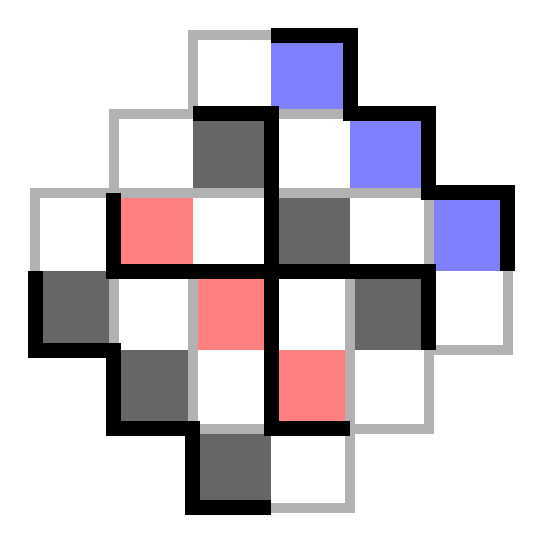
\begin{tikzpicture}


\sq{blue!50!white}{0}{2}
%\wsq{-1}{2}

\sq{blue!50!white}{ 1}{ 1}
%\wsq{ 0}{ 1}
\gsq{-1}{ 1}
%\wsq{-2}{ 1}

\sq{blue!50!white}{2}{0}
%\wsq{1}{0}
\gsq{0}{0}
%\wsq{-1}{0}
\sq{red!50!white}{-2}{0}
%\wsq{-3}{0}

%\wsq{ 2}{-1}
\gsq{ 1}{-1}
%\wsq{ 0}{-1}
\sq{red!50!white}{-1}{-1}
%\wsq{-2}{-1}
\gsq{-3}{-1}

%\wsq{ 1}{-2}
\sq{red!50!white}{ 0}{-2}
%\wsq{-1}{-2}
\gsq{-2}{-2}

%\wsq{ 0}{-3}
\gsq{-1}{-3}

\draw[line width=0.05in, color=black!30!white] (0,0)--(2,0)--(2,1)--(0,1)--cycle;

\draw[line width=0.05in, color=black!30!white] (0,1)--(2,1)--(2,2)--(0,2)--cycle;

\draw[line width=0.05in, color=black!30!white] (-1,2)--(1,2)--(1,3)--(-1,3)--cycle;

\draw[line width=0.05in, color=black!30!white] (2,1)--(3,1)--(3,-1)--(2,-1)--cycle; 

\draw[line width=0.05in, color=black!30!white] (-2,2)--(0,2)--(0,1)--(-2,1)--cycle;

\draw[line width=0.05in, color=black!30!white] (-2,1)--(0,1)--(0,0)--(-2,0)--cycle;

\draw[line width=0.05in, color=black!30!white] (-3,1)--(-2,1)--(-2,-1)--(-3,-1)--cycle; 

\draw[line width=0.05in, color=black!30!white] (-2,-2)--(-1,-2)--(-1,0)--(-2,0)--cycle;

\draw[line width=0.05in, color=black!30!white] (-1,-2)--( 0,-2)--( 0,0)--(-1,0)--cycle;

\draw[line width=0.05in, color=black!30!white] ( 0,-2)--( 1,-2)--( 1,0)--( 0,0)--cycle;

\draw[line width=0.05in, color=black!30!white] ( 1,-2)--( 2,-2)--( 2,0)--( 1,0)--cycle;

\draw[line width=0.05in, color=black!30!white] (-1,-3)--(1,-3)--(1,-2)--(-1,-2)--cycle;

\draw[line width=0.075in] (-2,1)--(-2,0)--(-1,0)--(0,0)--(0,-1)--(0,-2)--(1,-2);

\draw[line width=0.075in] (0,3)--(1,3)--(1,2)--(2,2)--(2,1)--(3,1)--(3,0);

\draw[line width=0.075in] (-1,2)--(0,2)--(0,1)--(0,0)--(1,0)--(2,0)--(2,-1);

\draw[line width=0.075in] (-3,0)--(-3,-1)--(-2,-1)--(-2,-2)--(-1,-2)--(-1,-3)--(0,-3);

\end{tikzpicture}
\end{center}
Exercise 5: prove limiting behavior of zig-zag

\newpage

\noindent The Krawtchouk ensemble is the correct ensemble for the Aztec Diamond problem.  We only focus on $p = \frac{1}{2}$:
$$ \mathbb{P}_{\text{Kr}}[(h_1, \dots h_n)]= \frac{1}{Z} \times \frac{1}{2^{\binom{N}{2}}} \times \Delta_N(h) \times  \prod_{j=1}^N \binom{K}{h_j} $$ 
where the normalization $Z$ is a number:
$$ \frac{N!}{0!\times 1!\times 2!\times \dots \times (N-1)!} \times \frac{1}{2^{\binom{N}{2}}} \times \prod_{j=1}^N \binom{K}{j} $$
the meaning of these number would be clear to a professor Combinatorics\footnote{or various branches of Computer Science} these are related to the Krawtchouk polynomials.  \\ \\
Johansson attributes the circular shape o Timo Sepalainen.  We settle for this summary by Persi Diaconis and Robert Griffiths
\begin{quotation}
\color{black!60!white}{Orthogonal polynomials for the multinomial distribution of N balls dropped into d boxes  are called multivariate Krawtchouk polynomials.}
\end{quotation}
These ball-and-urn models are commonplace.

\newpage

\noindent The limit shape seems to be known from the theory of \textbf{first-passage percolation}.  It would not hurt to read the book by Grimmett.
$$ 
\mu(x,y) = 
\left\{ 
\begin{array}{ll} 
y & \text{if }x < y \\
y + (\sqrt{x/2} + \sqrt{y/2})^2 & \text{if }x \geq y
\end{array}
 \right.
$$
The earliest proof by Jockusch-Shor-Propp uses the TASEP model\footnote{which can be converted to this type of ``first-passage percoltion".  More on this once I figure it out.} \\ \\ 
The most important is that we have a formula for all possible $\vec{h}$ on a given row (and later, the joint probability density over all rows). \\ \\ Johansson says it is an easy analysis from here.

\newpage

\noindent \textbf{2} - Determinantal Processes \\ \\
The surprising fact that\footnote{The surprising fact that there is any formula at all \dots}:
$$ \mathbb{P}(h)
= \frac{1}{Z_M \, 2^{\binom{M}{2}}} \prod_{1 \leq i < j \leq M}
(h_i - h_j)^2 \prod_{k=1}^M
\binom{M}{k}
 $$
I could not figure out the ball-and-urn model this is associated to this combination formula. \\ \\
The theory of determinantal processes says once we know the kernel we know everything else about that process\footnote{The theory of determinantal processes - especially the \textbf{geometry} - will be important once I assemble the basic discussion.}.  The Krawtchouk polynomials are orthogonal with respect to:
$$ \frac{1}{2^N} \binom{N}{x} =
  \frac{1}{2^N} \binom{N}{\frac{N}{2} + t \sqrt{N}} \to \frac{1}{2\pi } e^{-t^2 / 2}$$
if $ x = \frac{N}{2} + t \sqrt{N}$ were we magically know the correct scaling :-) \\ \\
The probabilities are \textbf{Slater determinant} of the different wave functions:
$$ \mathbb{P}[h] = \det \Big[ \sum \psi_n(h_i)\psi_n(h_j) \Big]_{i,j}$$

\newpage

\noindent A kind of smart-alec way of finding the Kernel is to say: $K(x,y) = \sum_{n=1}^N \psi_n(x)\psi_n(y)$ equal to

$$ 
\oint dz \; (1+qz)^x(1-pz)^{N-x}
(1+q\overline{z})^y(1-p\overline{z})^{N-y}
$$
Then the particle density would be if we set $x = y$:
$$ \rho(x) =
\oint dz \; \Big|(1+z/2)^x(1-z/2)^{N-x}\Big|^2
 $$
 and I had better hope the middle coefficient convergest to the semicircle:
 $$ \rho(x) = \frac{1}{\pi}\sqrt{1-x^2}$$
Oh it seems we have bypassed the Gaussians.  \\ \\
Oops if we define Krawtchouk polynomials by:
$$ \sum_{n=0}^N \psi_n(x) \frac{z^n}{n!} = (1+z/2)^x (1-z/2)^{N-x} $$
then the formula we have written is different from 
$\sum \psi_n(x) \psi_n(y)$ instead it's $\frac{1}{n!^2}\sum \psi_n(x) \psi_n(y)$.  And it's $\text{length}^\text{2}$ will be:
$$ \frac{1}{2^{2n}}\binom{N}{n} $$
\newpage

\noindent These definitions are so confusing.  I may have to start from scratch. \\ \\
\textbf{3} - Determintanal Processes  \\ \\
In this iteration, we try to become accountable for the formulas we use, and making sure they represent what we want. \\ \\
What ever the Krawtchuk polynomials are there is a formula for them here:
$$ \sum_{n=0}^N K_n (x; N, p) \frac{z^n}{n!} 
= (1+qz)^x (1 - pz)^{N-x} $$
For simplicity I am going to set $p = q = \frac{1}{2}$ .  What does $N = 2$ look like?
\begin{eqnarray*} K_0(x) + K_1(x)z + K_2(x) \frac{z^2}{2}
&=& (1+\tfrac{1}{2}z)^x (1 - \tfrac{1}{2}z)^{2-x} \\
&=& ? \end{eqnarray*}
If we expand to $x$ places that doesn't simplify very much now, does it?   \newpage

\noindent Here is another version:
$$ \sum_{n=0}^N Q_n(x) z^n = (1 - z)^x(1+z)^{N-x} $$
with duality $Q_n(x) = Q_x(n)$.  Does it matter if we use $K$ or $Q$? \\ \\
Here is the formula again:
$$ \mathbb{P}(h)
= \frac{1}{Z_M \, 2^{\binom{M}{2}}} \prod_{1 \leq i < j \leq M}
(h_i - h_j)^2 \prod_{k=1}^M
\binom{M}{k}
 $$
and I could set $M = 3$:
$$ \mathbb{P}(h) = \left|
\begin{array}{ccccc}
1 \binom{3}{1} & &\frac{1}{2}a \binom{3}{2}& &\frac{1}{2^2}a^2 \binom{3}{3}\\ \\
1 \binom{3}{1}& &\frac{1}{2}b \binom{3}{2}& &\frac{1}{2^2}b^2 \binom{3}{3}\\ \\
1 \binom{3}{1}& &\frac{1}{2}c \binom{3}{2}& &\frac{1}{2^2}c^2 \binom{3}{3}\\
 \end{array}
 \right| $$
Then using row operations (such as Gram-Schmidt) we can pain-stakingly make these three columns orthogonal with respect to $w(x) = \binom{N}{x}\frac{1}{2^N}$

\newpage

If we look at the formula at let $n$ be random
$$\mathbb{E}[ K_n(x,N) ] = \sum_{n=0}^N K_n (x; N) \frac{z^n}{n!} 
= (1+z/2)^x (1 - z/2)^{N-x} $$
in the limit $n \to \infty$ $\mathbb{P}(n) = \frac{z^n}{n!}$ is a Poisson distribution, with average $z$. \\ \\
$\ast$ We are still learning, let's use the simpliest formula: let $X = \xi_1 + \dots + \xi_n $
$$ G(z; X) = \prod_{j=1}^N \big(1 + u(\xi_j)z\big) $$
and the Krawtchuk polynomials simply fall out:
$$ K_n(X) = n! \sum_{\sigma \in S_n} u(\xi_{\sigma(1)})\dots u(\xi_{\sigma(1)}) $$
This notation is getting hard to read -- \textbf{defeating the purpose of notation}. The $\xi \in \{ 0,1\}$ so that $u(\xi) = \xi - \frac{1}{2} \in \{ \frac{1}{2}, - \frac{1}{2}\}$.
$$ K_n(X) = n! \sum_{\sigma \in S_N} (-1)^{f(\sigma, n, N)} \frac{1}{2^n} $$
for some indeterminate function $f$.  I think\footnote{when do we have a formula in real life?  never!}

\newpage

\noindent Since I have no idea what I am doing let's try:
$$ Q_n(x) = \sum_{k = 0}^N \frac{\binom{x}{k}\binom{N-x}{n-k}}{\binom{N}{n}}
= \sum_{k = 0}^N \frac{\binom{n}{k}\binom{N-n}{x-k}}{\binom{N}{x}} $$
then we are trying to evaluate a very complicated determinant:
$$ \det \Bigg[ 
\sum_{n=0}^N \bigg(
\sum_{k = 0}^N \frac{\binom{n}{k}\binom{N-n}{x_i-k}}{\binom{N}{x_i}} \times 
\sum_{k = 0}^N \frac{\binom{n}{k}\binom{N-n}{x_j-k}}{\binom{N}{x_j}}\bigg)
\Bigg]_{i,j} $$
again this is pretty dreadful to read and we don't know what these objects are counting.
$$ \det \left[ \sum_{n=0}^N Q_n(x_i) Q_n(x_j)\right]_{i,j}$$
This is simpler but less informative.  

\newpage

\noindent \textbf{4} - The Ehrenfest Urn model.  \\ \\
In a way the Krawtchouk polynomials are pretty stupid.  They are orthogonal to the binomial coefficients:
$$ \sum_{x=0}^N \psi_m(x) \psi_n(x) \times \frac{1}{2^N} \binom{N}{x} = \left\{
\begin{array}{cl} 0 & \text{if }m \neq n \\
? & \text{otherwise}\end{array}
 \right.$$
but actually the steady state of a random walk on $\{ 0, \dots, N\}$ with odds of jumping half to the left and to the right, is the uniform distribution.  \\ \\
This is known was the \textbf{gambler's ruin}.  Instead we need the Ehrenfest urn model.  

\begin{quotation}
An urn has $N$ balls coloured {\color{red}{red}} or {\color{blue}{blue}}. Transitions in a Markov chain
are made by selecting a ball at random and changing its colour. $X_t$
is the
number of red balls after $t$ transitions. \\ \\ $\{X_t\}_t \in \mathbb{N}$ is a reversible Markov Chain
with a Binomial $(N, \frac{1}{2})$ stationary distribution. \end{quotation}

\newpage

\noindent This can also be considered a random walk on $(\mathbb{Z}_2)^N$.

\newpage

\fontfamily{qag}\selectfont \fontsize{12}{10}\selectfont

\begin{thebibliography}{}

\item Kurt Johansson \textbf{Discrete orthogonal polynomial ensembles and the Plancherel measure.} \texttt{math/9906120} Annals of Mathematics (2) 153 (2001), No. 2, 259--296.

\item Benjamin J. Fleming, Peter J. Forrester.  \textbf{Interlaced particle systems and tilings of the Aztec diamond.} \texttt{arXiv:1004.0474}

\item Manuel Fendler, Daniel Grieser.	 \textbf{A new simple proof of the Aztec diamond theorem.}  \texttt{arXiv:1410.5590} 

\item Fr\'{e}d\'{e}ric Bosio, Marc A. A. Van Leeuwen.  \textbf{A bijection proving the Aztec diamond theorem by combing lattice paths.} \texttt{arXiv:1209.5373}

\item David E. Speyer \textbf{Variations on a theme of Kasteleyn, with application to the totally nonnegative Grassmannian} \texttt{arXiv:1510.03501}

\item Persi Diaconis, Robert Griffiths.  \textbf{An introduction to multivariate Krawtchouk polynomials and their applications} \texttt{arXiv:1309.0112}

\item Tom Koornwinder \textbf{Krawtchouk Polynomials, a Unification of Two Different Group Theoretic Interpretations}
\texttt{SIAM J. Math. Anal., 13(6), 1011–1023.}

\item Richard Feynman \textbf{Statistical Mechanics} 

\end{thebibliography}

\newpage

\newpage

\fontfamily{qag}\selectfont \fontsize{20}{20}\selectfont

``The historically first example of such a system goes back to \textbf{De Moivre} (1738) and
\textbf{Laplace} (1812) who considered the problem of finding the asymptotic distribution of a sum
of i.i.d. random variables for Bernoulli trials, when the pre-limit distribution is explicit,
and took the limit of the resulting expression. \\ \\ 
\indent While this computation may look like a
simple exercise when viewed from the heights of modern probability, in its time it likely
served the role of a key stepping stone - {\color{blue!50!white!80!black}{first rigorous proofs of central limit theorems
appeared only in the beginning of the XXth century}}. \\ \\
\indent At the moment we are arguably in a ``De Moivre-Laplace stage" for a certain class
of stochastic systems which is often referred to as the \textbf{KPZ universality class}, after an
influential work of Kardar-Parisi-Zhang in mid-80's\dots" \\ \\

\fontfamily{qag}\selectfont \fontsize{25}{30}\selectfont
\noindent taken from: \\ \\
\fontfamily{qag}\selectfont \fontsize{20}{15}\selectfont
Alexei Borodin, Vadim Gorin.  \textbf{Lectures on Integrable probability} \texttt{1212.3351}


\end{document}